\documentclass[11pt]{article}

\usepackage[a4paper,margin=1in]{geometry}
\usepackage[T1]{fontenc}
\usepackage[utf8]{inputenc}
\usepackage{lmodern}
\usepackage{microtype}
\usepackage{amsmath,amssymb,amsthm,mathtools}
\usepackage{booktabs}
\usepackage{graphicx}
\usepackage{float}
\usepackage{placeins}
\usepackage{enumitem}
\usepackage[numbers,sort&compress]{natbib}
\usepackage{xcolor}
\usepackage{xurl}
\usepackage[colorlinks=true,linkcolor=blue!55!black,citecolor=blue!55!black,urlcolor=blue!55!black]{hyperref}
\usepackage[nameinlink,noabbrev]{cleveref}

\setlength{\parindent}{1.4em}
\setlength{\parskip}{0.15em}
\setlist{itemsep=0.25em,topsep=0.35em}

\newtheorem{theorem}{Theorem}[section]
\newtheorem{proposition}[theorem]{Proposition}
\newtheorem{lemma}[theorem]{Lemma}
\newtheorem{corollary}[theorem]{Corollary}
\theoremstyle{definition}
\newtheorem{definition}[theorem]{Definition}
\theoremstyle{remark}
\newtheorem{remark}[theorem]{Remark}

\newcommand{\R}{\mathbb R}
\newcommand{\C}{\mathbb C}
\newcommand{\uc}{u_{\mathrm c}}
\newcommand{\Id}{\mathrm I}
\newcommand{\cK}{\mathcal K}
\newcommand{\cT}{\mathcal T}
\newcommand{\cR}{\mathcal R}
\newcommand{\cB}{\mathcal B}
\newcommand{\cC}{\mathcal C}
\newcommand{\cE}{\mathcal E}
\newcommand{\cH}{\mathcal H}
\newcommand{\cP}{\mathcal P}
\newcommand{\spec}{\operatorname{spec}}
\newcommand{\spr}{\operatorname{spr}}

\title{\textbf{Peripheral Biorthogonalization of Critical-Branch}\
\textbf{Returns at a Quadratic Band-Merging Map:}\\[0.35em]
\large Gauge Invariance, Branch-Memory Collapse, and a No-Go Theorem\\
for Normalization-Based Half Weights}
\author{Liang Wang\\
\small School of Artificial Intelligence and Automation,\\[-0.2em]
\small Huazhong University of Science and Technology, Wuhan 430074, P.R. China\\
\small \texttt{wangliang.f@gmail.com}}
\date{July 2026}

\begin{document}

\maketitle

\begin{abstract}
At the first algebraic band-merging parameter of $f_u(x)=1-u x^2$, a
two-branch Gaussian return has an almost rank-one bright channel.  In the
exchange-symmetric limit, both a unit-modulus cubic phase and a positive
half-weight reproduce the modulus of one branch.  The previous analysis
left open whether the half-weight could be derived from Perron/parity-
biorthogonal Grushin entrance and exit maps.  We give a negative answer to
that specific mechanism and identify a separate conditioning barrier.

Let $R,L$ collect biorthonormal right and left peripheral modes, and put
$Q=\Id-RL^*$.  For raw trial and test maps $V_0,W_0$, we prove that
\[
 G=W_0^*QV_0,
 \qquad V=QV_0,
 \qquad W^*=G^{-1}W_0^*Q
\]
give the canonical peripheral pair whenever $G$ is invertible.  Then
$W^*V=\Id$, $QV=V$, $W^*Q=W^*$, and $VW^*$ is an idempotent packet
projection inside the bulk complement.  Every invertible change of
biorthogonal coordinates acts on the reduced matrix by similarity.  It
preserves the endpoint operator, determinant, and nonzero spectrum and
therefore cannot divide a bright eigenvalue by two.

The dual to the unnormalized symmetric branch vector is indeed
$\frac12(1,1)$ under exact exchange symmetry.  Together with the synthesis
vector $(1,1)^T$, however, it forms the bright projector
$\frac12\left(\begin{smallmatrix}1&1\\1&1\end{smallmatrix}\right)$, which
acts as the identity on the bright range.  Inserting one half into the
physical return is an attenuation, not a coordinate normalization.  We also
show that real, static peripheral data produce a real bright reduction; a
nonreal cubic multiplier requires a spectral-parameter boundary condition
or another genuinely complex structure.

For two normalized branch histories with overlap $c$, their synthesis has
singular values $\sqrt{1\pm c}$.  Consequently every exact two-label dual
satisfies
\[
 \|W^*\|\ge(1-c)^{-1/2},
 \qquad
 \kappa(V^*V)=\frac{1+c}{1-c}.
\]
Seven-noise computations show progressive branch-memory collapse.  At
$\sigma=10^{-4}$, the endpoint overlap is $0.99885850$ and the raw Gram
condition is $1751.07$.  Peripheral projection increases the overlap to
$0.99906159$ and the condition to $2130.26$; the canonical analysis norm is
$32.72$.  At the critical slice itself, the complement Gram condition is
only $1.0145$ and the bright coordinate dual is
$(0.4999905,0.5000095)$.  Thus branch splitting is locally stable, but
closing two independent labels is not.  The correct next object is a
spectral-parameter bright/dark Schur complement whose self-energy can
genuinely attenuate and complexify the bright channel.
\end{abstract}

\noindent\textbf{Keywords:} Gaussian transfer operator; biorthogonal
projection; Grushin problem; branch memory; singular value; gauge
invariance; Schur complement; non-normal spectrum; quadratic map.

\medskip
\noindent\textbf{MSC 2020:} 37E05; 37D25; 47A10; 47A55; 47B65; 65F35;
65P30.

\section{Introduction}
\label{sec:introduction}

The small-noise spectrum of a Gaussian perturbation of a quadratic
band-merging map has been reduced through several increasingly local
operator models.  The deterministic bulk determinant has an exact endpoint
pole, Gaussian noise resolves a growing cloud, and endpoint singular values
supply a half-logarithmic clock
\citep{WangBulkScattering2026,WangEndpointRank2026}.  A boundary word then
gives a time-ordered cycle, while Riccati packets and a conditioned critical
profile realize that cycle inside the exact noisy operator
\citep{WangTimeOrdered2026,WangGaussianReturn2026}.

Two later tests changed the proposed completion mechanism.  The first showed
that the second critical preimage is an order-one channel and that a
sector-free time lift only replicates physical eigenvalues by Floquet
rotations \citep{WangComplement2026}.  The second reorganized the critical
slice as an exact two-branch factorization
\begin{equation}\label{eq:intro-factorization}
 \cR(\theta)=\cE J_\theta\cC,
 \qquad
 \cB(\theta)=J_\theta\cC\cE,
 \qquad
 J_\theta=\operatorname{diag}(1,e^{i\theta}),
\end{equation}
and proved equality of their nonzero spectra and Fredholm determinants
\citep{WangSectorBranch2026}.  In a rank-one exchange-symmetric model, the
only nonzero return eigenvalue is
\begin{equation}\label{eq:intro-rank-one}
 \eta(1+e^{i\theta}).
\end{equation}
Unit-modulus branch weights preserve one-branch modulus only at
$\theta=\pm2\pi/3$.  A positive half-weighted sum has the same modulus,
however.  Radius data cannot distinguish the two.

The most economical proposed source of the half-weight was dual
normalization.  A Grushin problem uses separate synthesis and analysis maps,
so the dual to the unnormalized bright vector $(1,1)^T$ is naturally
$\frac12(1,1)$.  Could this be the missing factor?  The answer is no.  A
proper dual normalization is an idempotent coordinate projection or an
invertible gauge.  It cannot change a nonzero eigenvalue.  The number one
half appears, but it is paired with a synthesis vector of norm two in branch
coordinates and causes no physical attenuation.

This no-go result is accompanied by a geometric obstruction.  The two
critical lobes are initially disjoint, but after they traverse the common
packet cycle their normalized histories become almost parallel.  An exact
two-label analysis map must then reconstruct a vanishing dark difference.
Its norm necessarily diverges.  Perron/parity projection does not restore
the lost branch memory in the computed tail; it makes the final overlap
slightly closer to one.

\subsection*{Main results and logical status}

\begin{enumerate}[label=\textbf{B\arabic*.},leftmargin=3.2em]
 \item \textbf{Canonical peripheral pair.}
 For every invertible complement Gram matrix, we construct exact trial and
 dual maps inside the oblique Perron/parity complement.  The associated
 packet projection is idempotent and compatible with the global bulk
 projection.

 \item \textbf{Biorthogonal gauge theorem.}
 Every invertible change of branch coordinates transforms the reduced matrix
 by similarity and leaves the endpoint return unchanged.  Hence ordinary
 dual normalization cannot supply a factor one half in the physical return.

 \item \textbf{Bright-projector no-go theorem.}
 The symmetric coordinate dual is exactly a half-sum, but its synthesis--
 analysis product is the bright projector.  On a bright invariant range it
 is the identity.  The operator that actually halves the return is not a
 projection.

 \item \textbf{Static-real limitation.}
 Real Gaussian dynamics, real peripheral projectors, and static real
 trial/test maps give a real reduced bright scalar.  A cubic relative phase
 is not produced by this algebra.  This does not disprove a cubic phase in a
 complex spectral-parameter closing map.

 \item \textbf{Branch-memory conditioning theorem.}
 If normalized branch histories have overlap $c$, their dark singular value
 is $\sqrt{1-c}$ and every exact two-label dual has norm at least
 $(1-c)^{-1/2}$.  Thus branch-memory collapse forbids a uniformly bounded
 two-label Grushin analysis.

 \item \textbf{Seven-noise audit.}
 The endpoint overlap rises from $0.65084$ to $0.99886$ across the archived
 scales, while the normalized Gram condition rises from $4.73$ to $1751$.
 These are floating-point diagnostics; no asymptotic convergence theorem is
 claimed.

 \item \textbf{Peripheral and gauge audit.}
 At $\sigma=10^{-3}$ and $10^{-4}$, exact sparse Perron/parity projectors
 satisfy residuals below $4.0\times10^{-15}$.  Canonical pair identities hold
 below $7.4\times10^{-14}$ and a nontrivial gauge similarity holds below
 $3.5\times10^{-17}$.  Peripheral extraction does not close the remaining
 gap to the physical bulk edge.
\end{enumerate}

The corrected implication diagram is
\begin{equation}\label{eq:logical-diagram}
 \boxed{
 \begin{gathered}
 \text{peripheral biorthogonalization}
 \Longrightarrow
 \text{exact bulk-compatible packet projection},\\
 \text{dual half-sum}
 \not\Longrightarrow
 \text{half-weighted physical return},\\
 \text{real static compression}
 \not\Longrightarrow
 \text{cubic branch phase},\\
 \text{branch-memory collapse}
 \Longrightarrow
 \text{ill-conditioned exact dark dual},\\
 \text{spectral bright/dark Schur map}
 \Longrightarrow?\
 \text{physical effective determinant}.
 \end{gathered}}
\end{equation}
The first four statements are proved here.  The final arrow is the next
operator problem.

\section{Gaussian operator and peripheral complement}
\label{sec:setup}

Let $\uc$ be the root in $(1,2)$ of
\begin{equation}\label{eq:cubic-parameter}
 u^3-2u^2+2u-2=0,
\end{equation}
and put
\begin{equation}\label{eq:map}
 f(x)=1-\uc x^2,
 \qquad
 \uc=1.543689012692076\ldots.
\end{equation}
For noise $\sigma>0$, the row-normalized folded Gaussian kernel is
\begin{align}
 P_\sigma(x,y)
 &=\frac{\phi_\sigma(y-f(x))+\phi_\sigma(y+f(x))}{Z_\sigma(x)},
 \label{eq:kernel}\\
 Z_\sigma(x)
 &=\int_0^1\{\phi_\sigma(y-f(x))+\phi_\sigma(y+f(x))\}\,dy,
 \label{eq:normalizer}\\
 \phi_\sigma(t)&=\frac{1}{\sqrt{2\pi}\sigma}e^{-t^2/(2\sigma^2)}.
 \label{eq:normal-density}
\end{align}
Let $\cK_\sigma$ be the corresponding backward Markov operator on
$\cH=L^2(0,1)$ and write
\begin{equation}\label{eq:two-step}
 \cT_\sigma=\cK_\sigma^2.
\end{equation}
At fixed noise, $\cK_\sigma$ is Hilbert--Schmidt and $\cT_\sigma$ is trace
class.

Let $r_0,r_-$ and $\ell_0,\ell_-$ be right and left Perron/parity modes,
normalized by
\begin{equation}\label{eq:biorthogonal-modes}
 \ell_i^*r_j=\delta_{ij},
 \qquad i,j\in\{0,-\}.
\end{equation}
Collect them as
\begin{equation}\label{eq:R-L}
 R=(r_0,r_-),
 \qquad
 L=(\ell_0,\ell_-),
 \qquad
 L^*R=\Id_2.
\end{equation}
The oblique peripheral and bulk projections are
\begin{equation}\label{eq:Q}
 \Pi_{\rm per}=RL^*,
 \qquad
 Q=\Id-RL^*.
\end{equation}
They satisfy
\begin{equation}\label{eq:Q-identities}
 Q^2=Q,
 \qquad QR=0,
 \qquad L^*Q=0.
\end{equation}
Since these are spectral projectors,
\begin{equation}\label{eq:bulk-decomposition}
 \cK_\sigma
 =r_0\ell_0^*+\lambda_-r_-\ell_-^*+K_{\rm b},
 \qquad
 K_{\rm b}=Q\cK_\sigma Q.
\end{equation}
The projection is generally nonorthogonal.  Its left and right data must
therefore be carried separately \citep{Kato1995,TrefethenEmbree2005}.

Let $P_0,\ldots,P_{k-2}$ be the packet windows along the component cycle and
let $P_-,P_+$ be the two disjoint critical windows.  The exact branch
entrance and exit maps from RH-20 are denoted
\begin{equation}\label{eq:branch-maps}
 \cC:\cH_0\longrightarrow\cH_-\oplus\cH_+,
 \qquad
 \cE:\cH_-\oplus\cH_+\longrightarrow\cH_0.
\end{equation}
The positive branch-complete endpoint return is $\cE\cC$ and the reversed
branch monodromy is $\cC\cE$.  Their nonzero spectra agree by the
$AB$--$BA$ identity \citep{GohbergKrein1969}.

\section{Canonical peripheral biorthogonalization}
\label{sec:canonical-pair}

Let $V_0:\C^m\to\cH$ be a raw synthesis map and let
$W_0^*:\cH\to\C^m$ be a raw analysis map.  In the numerical construction,
their columns are packet profiles.  Define the complement Gram matrix
\begin{equation}\label{eq:complement-gram}
 G=W_0^*QV_0.
\end{equation}

\begin{theorem}[Canonical peripheral pair]
\label{thm:canonical-pair}
Suppose $G$ in \eqref{eq:complement-gram} is invertible.  Define
\begin{equation}\label{eq:canonical-pair}
 \boxed{
 V=QV_0,
 \qquad
 W^*=G^{-1}W_0^*Q.}
\end{equation}
Then
\begin{align}
 QV&=V,
 &W^*Q&=W^*,
 \label{eq:pair-in-Q}\\
 L^*V&=0,
 &W^*R&=0,
 \label{eq:pair-annihilation}\\
 W^*V&=\Id_m.
 \label{eq:pair-duality}
\end{align}
The finite-rank operator
\begin{equation}\label{eq:packet-projection}
 \cP=VW^*
\end{equation}
is an idempotent projection satisfying
\begin{equation}\label{eq:projection-compatible}
 \cP^2=\cP,
 \qquad
 Q\cP=\cP Q=\cP.
\end{equation}
\end{theorem}

\begin{proof}
Idempotence of $Q$ gives
\[
 W^*V
 =G^{-1}W_0^*Q^2V_0
 =G^{-1}G
 =\Id_m.
\]
Equations \eqref{eq:pair-in-Q}--\eqref{eq:pair-annihilation} follow from
$Q^2=Q$, $QR=0$, and $L^*Q=0$.  Therefore
\[
 \cP^2=V(W^*V)W^*=VW^*=\cP,
\]
and the two compatibility identities follow from
$QV=V$ and $W^*Q=W^*$.
\end{proof}

This is an oblique Petrov--Galerkin construction.  The invertibility and
conditioning of $G$ are the finite-dimensional inf--sup condition
\citep{BoffiBrezziFortin2013,Chatelin1983}.  The theorem removes the
Perron/parity modes in both right and left data before packet localization is
used as a reduced coordinate system.

For an operator $A$ with $A=QAQ$, the reduced matrix is
\begin{equation}\label{eq:reduced-matrix}
 M=W^*AV.
\end{equation}
The theorem does not assert that $\cP A\cP$ approximates $A$ in operator
norm.  It makes the finite projection algebra exact, so that approximation
and normalization are not conflated.

\section{Gauge invariance and the half-weight no-go theorem}
\label{sec:gauge}

Biorthogonal coordinates have a natural gauge freedom.

\begin{theorem}[Biorthogonal gauge invariance]
\label{thm:gauge}
Let $S\in\mathrm{GL}(m,\C)$ and set
\begin{equation}\label{eq:gauge-pair}
 V_S=VS,
 \qquad
 W_S^*=S^{-1}W^*.
\end{equation}
Then
\begin{equation}\label{eq:gauge-duality}
 W_S^*V_S=\Id_m,
 \qquad
 V_SW_S^*=VW^*,
\end{equation}
and the reduced matrix transforms by similarity,
\begin{equation}\label{eq:gauge-similarity}
 \boxed{M_S=S^{-1}MS.}
\end{equation}
Consequently its characteristic polynomial, determinant, trace powers, and
eigenvalues are invariant.
\end{theorem}

\begin{proof}
The first two identities follow by cancellation of $S$ and $S^{-1}$.  The
last follows from
\[
 W_S^*AV_S=S^{-1}(W^*AV)S.
\]
Similarity gives all spectral invariants.
\end{proof}

The same statement is visible directly in the exact branch factorization.
If
\begin{equation}\label{eq:branch-gauge}
 \cC_S=S^{-1}\cC,
 \qquad
 \cE_S=\cE S,
\end{equation}
then
\begin{equation}\label{eq:endpoint-gauge-invariance}
 \cE_S\cC_S=\cE\cC,
 \qquad
 \cC_S\cE_S=S^{-1}(\cC\cE)S.
\end{equation}
No reciprocal scaling of entrance and exit maps can change the endpoint
return or halve its bright eigenvalue.

\subsection{Why the canonical half-sum is not a path half-weight}

Put
\begin{equation}\label{eq:bright-dark-vectors}
 b=\begin{pmatrix}1\\1\end{pmatrix},
 \qquad
 d=\begin{pmatrix}1\\-1\end{pmatrix}.
\end{equation}
The coordinate dual to the unnormalized bright vector in the Euclidean
metric is
\begin{equation}\label{eq:bright-dual}
 \beta^*=\frac12(1,1),
 \qquad
 \beta^*b=1.
\end{equation}
Their synthesis--analysis product is
\begin{equation}\label{eq:bright-projector}
 P_{\rm b}=b\beta^*
 =\frac12\begin{pmatrix}1&1\\1&1\end{pmatrix},
 \qquad
 P_{\rm b}^2=P_{\rm b}.
\end{equation}

\begin{theorem}[Bright-projector no-go]
\label{thm:half-no-go}
Assume the branch entrance is bright and the exit annihilates the dark
channel,
\begin{equation}\label{eq:bright-invariance}
 P_{\rm b}\cC=\cC,
 \qquad
 \cE P_{\rm b}=\cE.
\end{equation}
Then the normalized bright quotient leaves the endpoint return unchanged:
\begin{equation}\label{eq:bright-quotient-unchanged}
 \boxed{\cE P_{\rm b}\cC=\cE\cC.}
\end{equation}
By contrast,
\begin{equation}\label{eq:actual-half-insertion}
 \cE\left(\frac12\Id_2\right)\cC
 =\frac12\cE\cC.
\end{equation}
The insertion $\frac12\Id_2$ is not a projection.  Therefore the physical
half-weight cannot be obtained from an idempotent bright quotient or an
invertible biorthogonal gauge.
\end{theorem}

\begin{proof}
Equation \eqref{eq:bright-quotient-unchanged} follows immediately from either
identity in \eqref{eq:bright-invariance}.  Equation
\eqref{eq:actual-half-insertion} is scalar linearity, while
$(\frac12\Id_2)^2=\frac14\Id_2\ne\frac12\Id_2$.
\end{proof}

The conclusion is narrow but decisive.  A half-weight could still arise
from determinant combinatorics, a Schur self-energy, or a non-conservative
boundary condition.  It cannot be justified by saying only that the dual of
$(1,1)^T$ is $\frac12(1,1)$.

For a general complement metric $G$, the metric dual row to $b$ is
\begin{equation}\label{eq:metric-bright-dual}
 \beta_G^*=\frac{b^*G}{b^*Gb}.
\end{equation}
If branch exchange symmetry gives
\begin{equation}\label{eq:exchange-metric}
 G=\begin{pmatrix}a&c\\c&a\end{pmatrix},
\end{equation}
then \eqref{eq:metric-bright-dual} again gives exactly
$\frac12(1,1)$.  This explains the numerical coefficients near one half
without turning them into physical path weights.

\section{A static real reduction does not generate a cubic phase}
\label{sec:realness}

\begin{proposition}[Static-real limitation]
\label{prop:realness}
Suppose $A,Q,V_0,W_0$ are real and the complement Gram matrix is invertible.
Then the canonical pair in \eqref{eq:canonical-pair} and the reduced matrix
$M=W^*AV$ are real.  Every real gauge preserves this property.  In
particular, a one-dimensional bright reduction obtained from these data is a
real scalar and cannot itself supply the nonreal multiplier
$e^{\pm2\pi i/3}$.
\end{proposition}

\begin{proof}
Matrix multiplication and inversion over an invertible real matrix remain
real.  The one-dimensional conclusion is immediate.
\end{proof}

A real matrix of dimension at least two can of course possess a complex
conjugate eigenpair.  The proposition does not forbid that.  It says that a
static real dual normalization does not derive a prescribed complex
\emph{relative branch coefficient}.  Such a coefficient can enter naturally
after complexifying the spectral parameter in a resolvent or imposing a
complex closing boundary condition.  The conditional cubic-phase theorem of
RH-20 remains a candidate for that later mechanism; it is neither proved nor
disproved here.

\section{Branch-memory collapse and the dark-dual barrier}
\label{sec:memory}

Let $u_-,u_+\in\cH$ be unit vectors representing two branch histories at the
same packet slice.  After a harmless phase choice, assume
\begin{equation}\label{eq:overlap}
 \langle u_-,u_+\rangle=c,
 \qquad0\le c<1.
\end{equation}
Define the synthesis
\begin{equation}\label{eq:history-synthesis}
 V_c=(u_-,u_+):\C^2\to\cH.
\end{equation}

\begin{theorem}[Exact branch-memory conditioning]
\label{thm:memory-conditioning}
The singular values of $V_c$ are
\begin{equation}\label{eq:history-singular-values}
 s_{\rm b}=\sqrt{1+c},
 \qquad
 s_{\rm d}=\sqrt{1-c}.
\end{equation}
Consequently
\begin{align}
 \kappa_2(V_c)
 &=\sqrt{\frac{1+c}{1-c}},
 \label{eq:synthesis-condition}\\
 \kappa_2(V_c^*V_c)
 &=\frac{1+c}{1-c}.
 \label{eq:gram-condition}
\end{align}
For every exact dual $W^*$ satisfying $W^*V_c=\Id_2$,
\begin{equation}\label{eq:dual-lower-bound}
 \boxed{\|W^*\|_2\ge\frac1{\sqrt{1-c}}.}
\end{equation}
Thus no uniformly bounded exact two-label analysis exists if $c\to1$.
\end{theorem}

\begin{proof}
The Gram matrix is
\[
 V_c^*V_c=\begin{pmatrix}1&c\\c&1\end{pmatrix},
\]
whose eigenvalues are $1+c$ and $1-c$.  This proves
\eqref{eq:history-singular-values}--\eqref{eq:gram-condition}.  Let
$e_{\rm d}=2^{-1/2}(1,-1)^T$.  Since $W^*V_c=\Id_2$,
\[
 1=\|e_{\rm d}\|
 =\|W^*V_ce_{\rm d}\|
 \le\|W^*\|\,\|V_ce_{\rm d}\|
 =\|W^*\|\sqrt{1-c},
\]
which gives \eqref{eq:dual-lower-bound}.
\end{proof}

The bright history $(u_-+u_+)/\sqrt2$ stays of order one, while the dark
history $(u_--u_+)/\sqrt2$ has norm $\sqrt{1-c}$.  Reconstructing the two
labels separately therefore amplifies perturbations in the vanishing dark
direction.  This is a conditioning statement, not an assertion that the
dark channel has no dynamical effect.  A small vector can be multiplied by a
large resolvent in a non-normal problem \citep{StewartSun1990,TrefethenEmbree2005}.

\subsection{Propagation from the critical split}

Let $\psi_-,\psi_+$ be the normalized disjoint critical profiles.  Starting
at the final slice, define recursively
\begin{align}
 h_{k-1}^\pm&=\psi_\pm,
 \label{eq:history-final}\\
 h_j^\pm&=P_j\cT_\sigma h_{j+1}^\pm,
 \qquad j=k-2,\ldots,0.
 \label{eq:history-recursion}
\end{align}
The normalized branch-memory overlap at slice $j$ is
\begin{equation}\label{eq:history-overlap}
 c_{\sigma,j}
 =\frac{|\langle h_j^-,h_j^+\rangle|}
 {\|h_j^-\|\,\|h_j^+\|}.
\end{equation}
At the critical slice, $c_{\sigma,k-1}=0$ because the supports are disjoint.
The endpoint value $c_{\sigma,0}$ measures how much branch identity survives
one restricted cycle before closing.

\subsection{Why peripheral projection need not separate merged histories}

\begin{proposition}[Stable projections preserve collapse]
\label{prop:projection-collapse}
Let $Q_n$ be bounded projections with $\sup_n\|Q_n\|<\infty$.  Suppose
$\|u_n^+-u_n^-\|\to0$ and
\begin{equation}\label{eq:projected-lower-bound}
 \min\{\|Q_nu_n^-\|,\|Q_nu_n^+\|\}\ge m>0.
\end{equation}
Then the normalized projected vectors also merge:
\begin{equation}\label{eq:projected-collapse}
 \left\|
 \frac{Q_nu_n^-}{\|Q_nu_n^-\|}
 -
 \frac{Q_nu_n^+}{\|Q_nu_n^+\|}
 \right\|\longrightarrow0.
\end{equation}
\end{proposition}

\begin{proof}
For nonzero vectors $x,y$ with norms at least $m$,
\[
 \left\|\frac{x}{\|x\|}-\frac{y}{\|y\|}\right\|
 \le\frac{2}{m}\|x-y\|.
\]
Apply this with $x=Q_nu_n^-$ and $y=Q_nu_n^+$, then use
$\|Q_n(u_n^--u_n^+)\|\le\|Q_n\|\|u_n^--u_n^+\|$.
\end{proof}

The proposition is conditional; uniform boundedness of the nonorthogonal
spectral projections is itself an issue in a singular limit.  It explains
why removing two global modes does not automatically recreate local branch
information already erased by the common packet dynamics.

\section{Numerical protocol}
\label{sec:protocol}

The analytic theorems above require no numerical assumptions.  The audit
tests three model-specific questions: whether branch histories merge across
the seven archived scales, whether peripheral projection reverses that
merger, and whether canonical normalization changes the reduced bright
eigenvalue.

We use the row-normalized folded midpoint matrices of RH-15--RH-20 with
\begin{equation}\label{eq:dimension-law}
 n\sigma=20.48
\end{equation}
and an eight-standard-deviation sparse Gaussian cutoff.  The component
period is
\begin{equation}\label{eq:period-selection}
 k=N_\sigma^{\rm H}+1,
\end{equation}
where $N_\sigma^{\rm H}$ is the independently computed Hellinger half-energy
rank from RH-16.  Every packet window uses the fixed multiple $L=6$.

The critical profiles are obtained by pulling back the endpoint Gaussian
once and splitting the resulting profile at the physical partition
$b=\uc^{-1/2}$.  Both columns are then propagated by
\eqref{eq:history-recursion}.  No profile projection is inserted between
packet masks, so the calculation retains the complete branch history inside
each window.

At $\sigma=10^{-3}$ and $10^{-4}$, sparse left and right Perron/parity modes
are resolved separately.  The canonical pair
\eqref{eq:canonical-pair} is constructed both at the critical slice and from
the normalized endpoint histories.  Four $2\times2$ cycle matrices are then
formed:
\begin{enumerate}[label=(\roman*),leftmargin=2.4em]
 \item raw dynamics with Euclidean critical profiles;
 \item raw dynamics with the canonical $Q$ pair;
 \item $K_{\rm b}^2$ inserted before every localization with Euclidean
 profiles;
 \item the same bulk dynamics with the canonical $Q$ pair.
\end{enumerate}
The full matrices are ordinary floating-point compressions.  They are not
operator-norm or pseudospectral enclosures.

\section{Seven-noise branch-memory audit}
\label{sec:seven-noise}

\begin{table}[H]
\centering
\small
\caption{Endpoint branch-memory collapse.  The Gram condition and dual lower
bound use individually normalized histories.  The final column is the
smaller/larger eigenvalue-modulus ratio of the closed two-profile return.}
\label{tab:memory-collapse}
\begin{tabular}{rrrrrr}
\toprule
$\sigma$ & $k$ & $c_{\sigma,0}$ & $\kappa(V^*V)$
& dual lower bound & return dark/bright\\
\midrule
$10^{-2}$        &3&0.650839&4.73&1.69&$4.07\times10^{-2}$\\
$4\times10^{-3}$ &4&0.875033&15.00&2.83&$2.00\times10^{-2}$\\
$2\times10^{-3}$ &5&0.970543&66.90&5.83&$2.70\times10^{-4}$\\
$10^{-3}$        &6&0.994092&337.52&13.01&$4.01\times10^{-5}$\\
$5\times10^{-4}$ &6&0.984404&127.24&8.01&$1.35\times10^{-2}$\\
$2\times10^{-4}$ &7&0.994965&396.22&14.09&$3.99\times10^{-3}$\\
$10^{-4}$        &8&0.998858&1751.07&29.60&$1.45\times10^{-5}$\\
\bottomrule
\end{tabular}
\end{table}

The clock staircase prevents monotonicity at every adjacent noise.  The
period stays at six between $10^{-3}$ and $5\times10^{-4}$, while the
critical clearance-to-noise ratio changes.  Nevertheless, the overall
pattern is strong.  Each additional cycle depth reduces the branch-memory
defect, and the cleanest smallest-noise point has a dark history singular
value
\begin{equation}\label{eq:smallest-dark-singular}
 \sqrt{1-c_{10^{-4},0}}=0.033786\ldots.
\end{equation}
Any exact two-label dual must therefore have norm at least $29.60$ before
peripheral projection.

The last column of \cref{tab:memory-collapse} is not determined solely by
$c_{\sigma,0}$.  It also depends on the final closing channel and branch norm
asymmetry.  Its small values at the most symmetric clock cells are consistent
with the same rank-one bright collapse, but no universal exponent is fitted.

\begin{figure}[t]
\centering
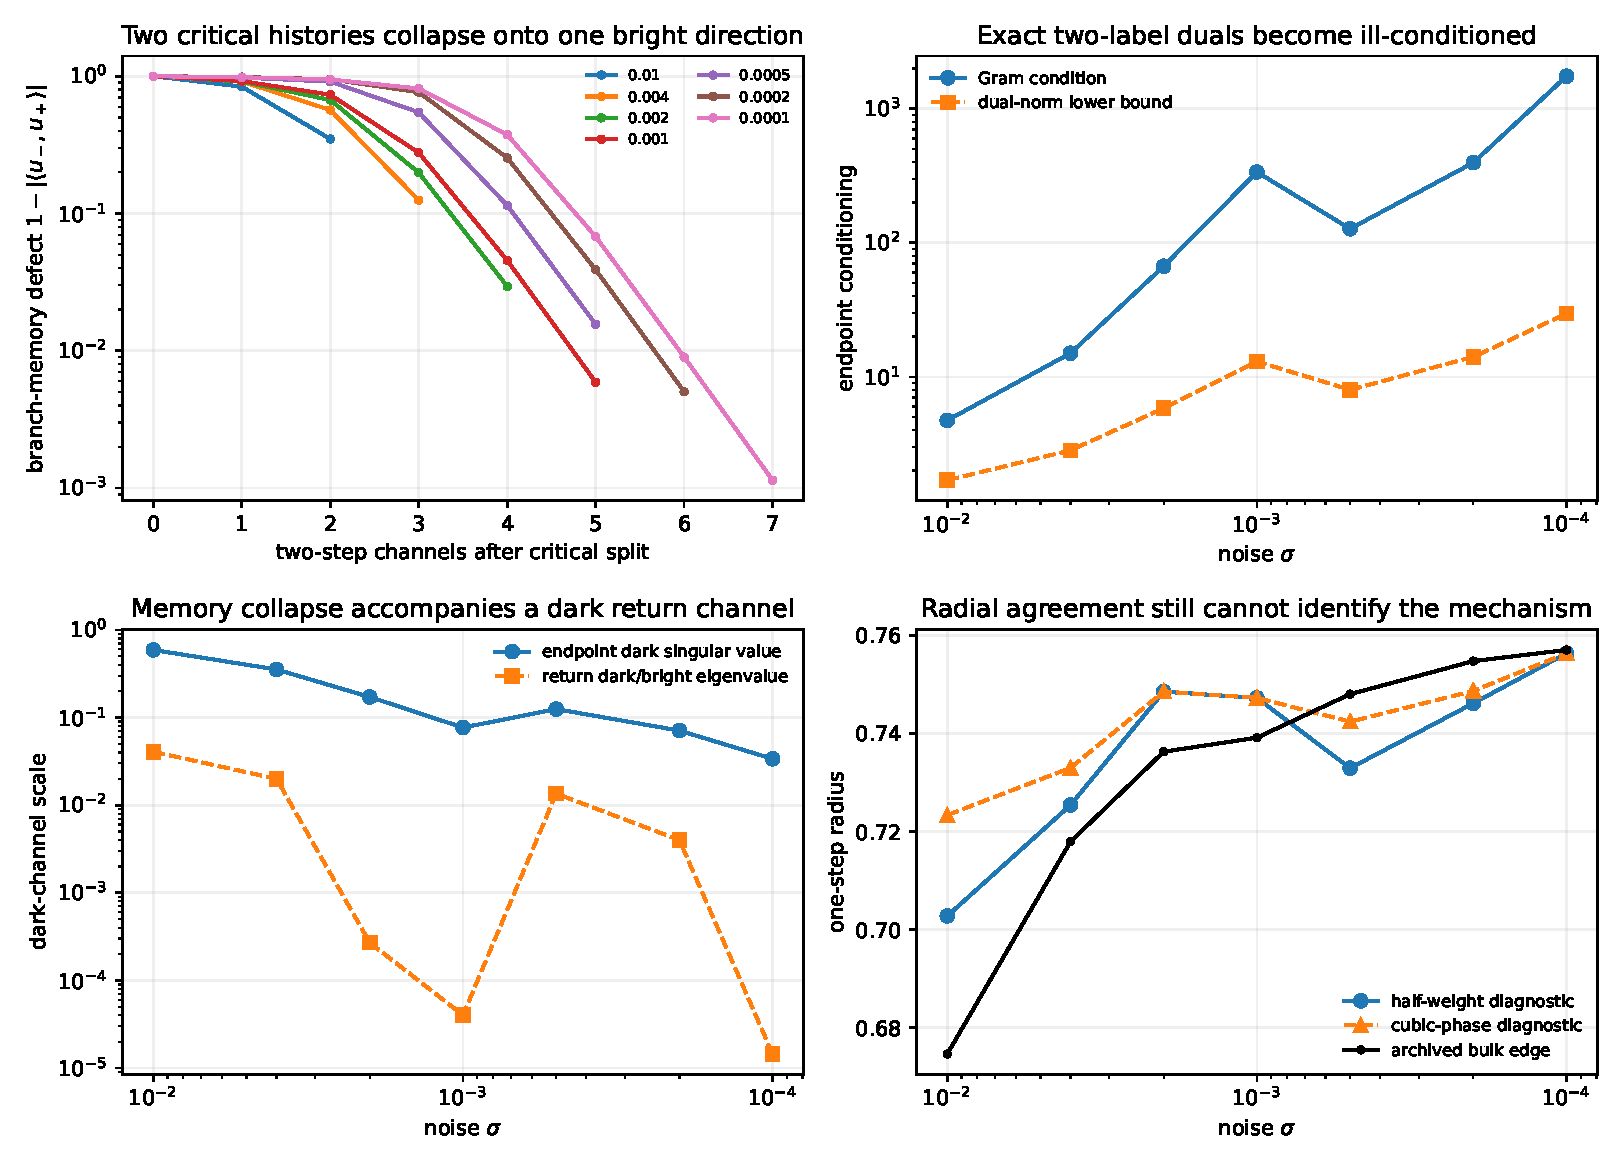
\includegraphics[width=0.92\textwidth]{figures/branch_memory_collapse.pdf}
\caption{Branch-memory audit.  Top left: the two initially disjoint critical
histories merge as they traverse the common packet cycle.  Top right: the
endpoint Gram condition and universal dual-norm lower bound.  Bottom left:
the endpoint dark singular value and the dark/bright eigenvalue ratio of the
closed return.  Bottom right: half-weight and cubic-phase radial diagnostics
remain nearly indistinguishable at branch-symmetric tail points.}
\label{fig:memory-collapse}
\end{figure}

The positive half-weight and cubic-phase scalar diagnostics at the smallest
noise are
\begin{equation}\label{eq:half-cubic-smallest}
 \rho_{1/2}=0.7563353896,
 \qquad
 \rho_{\rm cub}=0.7563358794,
 \qquad
 \rho_{\rm bulk}=0.7570230790.
\end{equation}
Their difference is below $5\times10^{-7}$.  This excellent radial
degeneracy is exactly why the gauge theorem is needed: a numerical radius
cannot turn a coordinate half-sum into a physical attenuation.

\section{Peripheral biorthogonal audit}
\label{sec:peripheral-audit}

\subsection{The critical pair is stable}

At the critical slice the raw profiles have disjoint support.  Peripheral
projection introduces a small overlap but leaves the complement Gram matrix
well conditioned.

\begin{table}[H]
\centering
\small
\caption{Canonical peripheral pairs at two representative noises.  The
critical coefficients are the metric bright dual in
\eqref{eq:metric-bright-dual}; the endpoint quantities use normalized
projected histories.}
\label{tab:peripheral-pairs}
\begin{tabular}{rrrrrrr}
\toprule
$\sigma$ & $\kappa(G_{\rm crit})$ & $\beta_-$ & $\beta_+$
& $c_{Q,0}$ & $\kappa(G_{Q,0})$ & $\|W_{Q,0}^*\|$\\
\midrule
$10^{-3}$&1.04594&0.499942&0.500058&0.995185&414.38&14.42\\
$10^{-4}$&1.01450&0.499991&0.500009&0.999062&2130.26&32.72\\
\bottomrule
\end{tabular}
\end{table}

At $\sigma=10^{-4}$, the critical complement metric is
\begin{equation}\label{eq:critical-metric-smallest}
 G_{\rm crit}=
 \begin{pmatrix}
 0.99282632&-0.00715497\\
 -0.00713512&0.99288349
 \end{pmatrix}.
\end{equation}
Its slight nonsymmetry comes from the oblique left/right peripheral
projection.  Equation \eqref{eq:metric-bright-dual} gives
\begin{equation}\label{eq:critical-bright-dual-smallest}
 \beta_G^*=(0.49999053,0.50000947).
\end{equation}
This is compelling evidence for an exchange-symmetric \emph{coordinate}
dual.  By \cref{thm:half-no-go}, it is not evidence that the physical return
contains the attenuation $\frac12\Id_2$.

\subsection{Peripheral extraction does not restore branch memory}

The endpoint histories become still more parallel after $Q$ is applied.  At
$\sigma=10^{-4}$,
\begin{align}
 c_{\rm raw}&=0.99885850,
 &\kappa(G_{\rm raw})&=1751.07,
 \label{eq:raw-memory-smallest}\\
 c_Q&=0.99906159,
 &\kappa(G_Q)&=2130.26.
 \label{eq:q-memory-smallest}
\end{align}
The universal lower bound for the normalized projected dual is $32.64$ and
the canonical analysis norm is $32.72$.  Thus the implementation is close to
the best possible norm for this trial space; the large value is geometric,
not a poor inversion algorithm.

The projected critical synthesis retains $99.76\%$ of its norm in the two
critical windows at $\sigma=10^{-4}$.  The projected endpoint histories
retain $89.69\%$ in the endpoint window.  Global projection introduces
visible tails, but the branch-memory conclusion is not caused by complete
delocalization.

\subsection{Reduced cycle radii and gauge check}

\begin{table}[H]
\centering
\small
\caption{One-step radii of four static two-profile cycle compressions.  ``Q
pair'' means the canonical peripheral synthesis/analysis maps.  ``Bulk''
means $K_{\rm b}^2$ is applied before every packet localization.}
\label{tab:cycle-radii}
\begin{tabular}{rrrrrr}
\toprule
$\sigma$ & raw & raw + Q pair & bulk & bulk + Q pair & physical bulk\\
\midrule
$10^{-3}$&0.791254&0.783898&0.761115&0.761319&0.739142\\
$10^{-4}$&0.789706&0.788348&0.782483&0.782493&0.757023\\
\bottomrule
\end{tabular}
\end{table}

Peripheral extraction changes the selected subspace and can therefore
change a compressed eigenvalue.  Once the subspace is fixed, however, the
gauge theorem is exact.  For the nontrivial matrix
\begin{equation}\label{eq:numerical-gauge}
 S=\begin{pmatrix}1.7&0.25\\-0.35&0.8\end{pmatrix},
\end{equation}
the largest observed error in
$M_S=S^{-1}MS$ is $3.47\times10^{-17}$.  All static reduced matrices have
zero imaginary entry to floating-point precision.  The largest canonical
pair residual is $7.33\times10^{-14}$.

At the smallest noise, the bulk biorthogonal radius remains
\begin{equation}\label{eq:remaining-radial-gap}
 0.782493-0.757023=0.025470
\end{equation}
above the archived physical edge.  Static peripheral biorthogonalization
does not solve the physical determinant problem.

\begin{figure}[t]
\centering
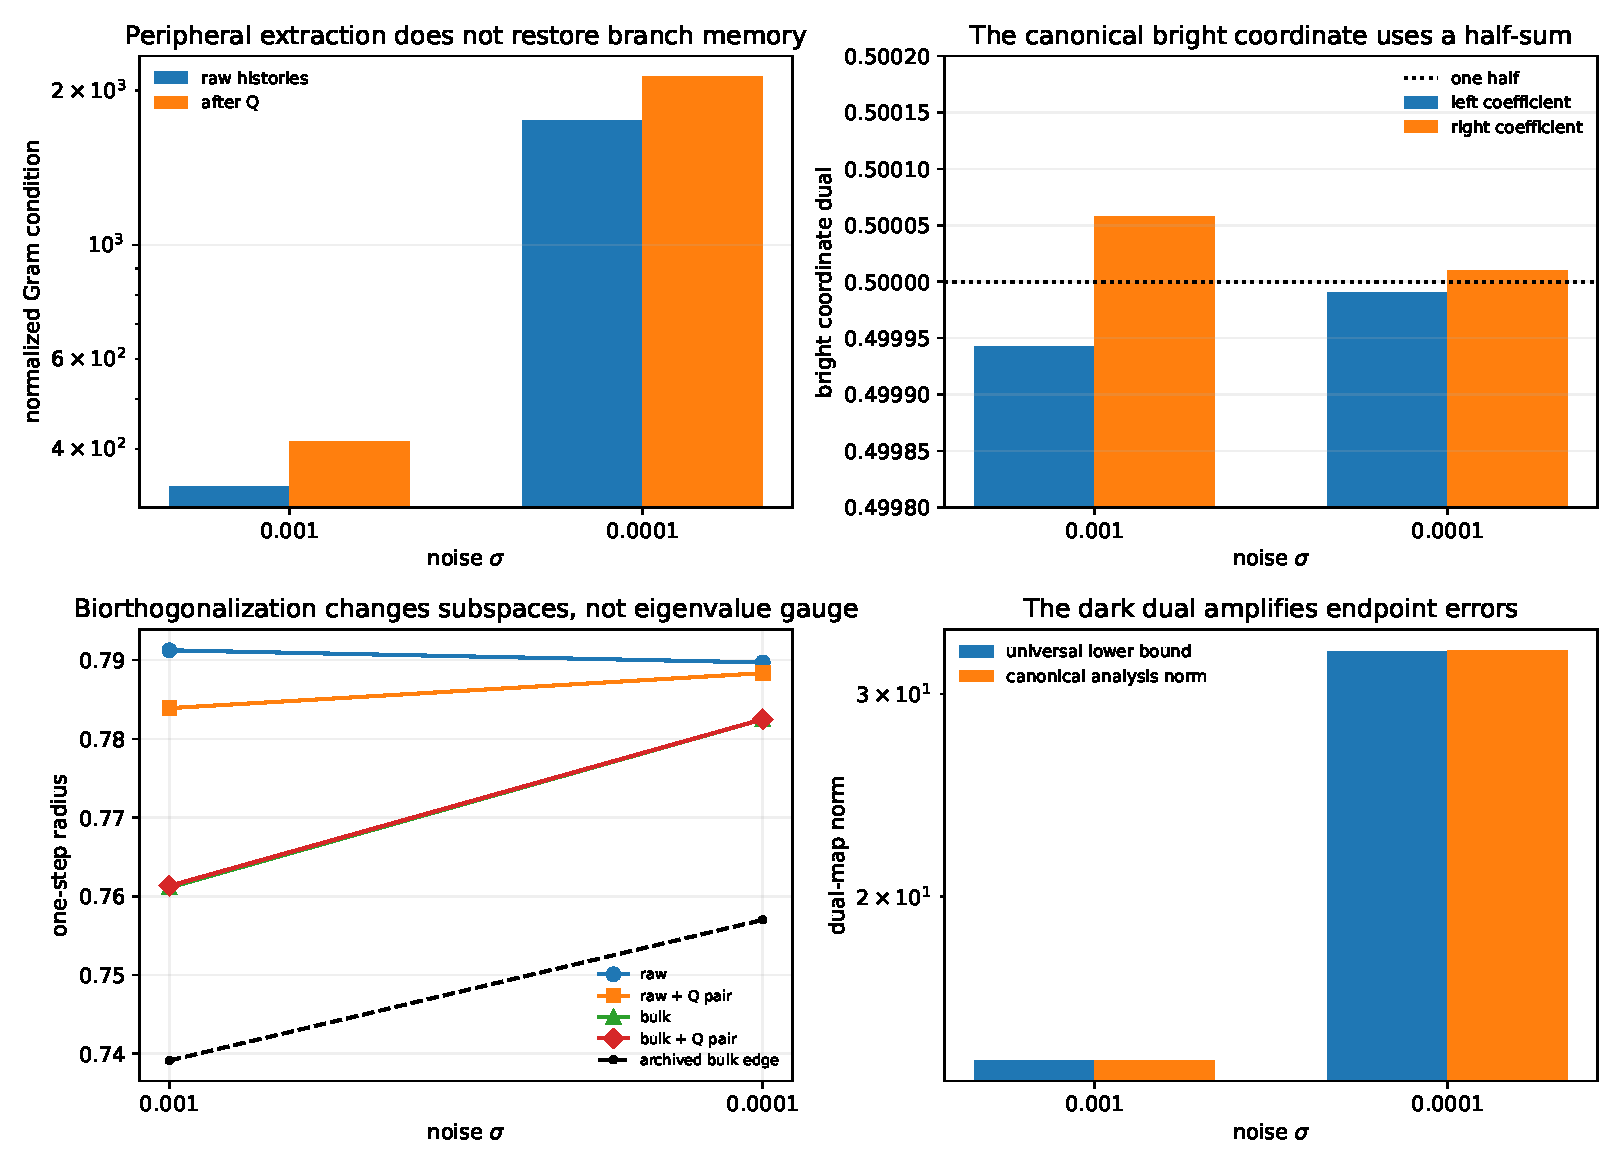
\includegraphics[width=0.92\textwidth]{figures/peripheral_biorthogonal_no_go.pdf}
\caption{Peripheral-biorthogonal audit.  Top left: endpoint branch-memory
conditioning before and after $Q$.  Top right: the critical bright coordinate
dual is nearly the exact half-sum.  Bottom left: static compressed cycle radii
remain above the physical bulk edge.  Bottom right: the canonical dark-dual
norm nearly saturates the universal lower bound.}
\label{fig:biorthogonal-audit}
\end{figure}

\subsection{Numerical status and reproducibility}

The implementation tests oblique complement idempotence, canonical left/right
annihilation, gauge similarity, the bright-projector no-go identity, exact
merge singular values, branch-history propagation, and cycle compression.
The audit records all intermediate overlaps, norms, Gram conditions, reduced
matrices, residuals, software versions, source hashes, and inherited-data
hashes.  NumPy, SciPy, and Matplotlib provide the numerical implementation
\citep{HarrisEtAl2020,VirtanenEtAl2020,Hunter2007}.  The largest sparse grid
has $n=204800$ midpoint cells.  No interval arithmetic, directed rounding,
operator-norm enclosure, or non-normal resolvent bound is used.

\section{The corrected next operator target}
\label{sec:next-target}

The static normalization gate gives a definite answer.  A canonical
peripheral pair exists and is stable at the critical split, but it neither
halves the bright return nor generates a complex phase.  Carrying two exact
labels around the cycle is also increasingly ill-conditioned.  The next
object should therefore eliminate the dark direction dynamically rather
than invert it as a permanent coordinate.

Let an exact or controlled branch effective matrix in the bright/dark basis
be
\begin{equation}\label{eq:z-effective-matrix}
 M(z)=
 \begin{pmatrix}
 M_{\rm bb}(z)&M_{\rm bd}(z)\\
 M_{\rm db}(z)&M_{\rm dd}(z)
 \end{pmatrix}.
\end{equation}
Whenever $z-M_{\rm dd}(z)$ is invertible, the scalar bright Schur map is
\begin{equation}\label{eq:bright-schur-map}
 \boxed{
 F_{\rm b}(z)
 =z-M_{\rm bb}(z)
 -M_{\rm bd}(z)
 \{z-M_{\rm dd}(z)\}^{-1}
 M_{\rm db}(z).}
\end{equation}
This operation is not a coordinate gauge.  Its self-energy is genuinely
$z$-dependent, can attenuate the real bright return, and becomes complex on
complex contours.  It is therefore capable in principle of producing
effects that \cref{thm:gauge,thm:half-no-go,prop:realness} rule out for a
static normalization \citep{SjoestrandZworski2007}.

A viable next analysis has four parts.
\begin{enumerate}[label=\textbf{D\arabic*.},leftmargin=3.1em]
 \item \textbf{Balanced bright/dark data.}
 Use the well-conditioned critical profiles to define bright and dark
 coordinates.  Do not reconstruct two nearly parallel endpoint histories
 as independent persistent labels.

 \item \textbf{Dark-channel Schur bound.}
 Estimate the three dark blocks in \eqref{eq:bright-schur-map} in a norm that
 includes the singular factor $\sqrt{1-c_{\sigma,0}}$.  Small dark vectors
 alone are insufficient; the dark resolvent must be controlled.

 \item \textbf{Spectral-parameter closing law.}
 Determine whether the resulting scalar self-energy is asymptotically real
 attenuation, a complex phase on the relevant contour, or neither.  No
 coefficient should be inserted from a radial fit.

 \item \textbf{Physical determinant comparison.}
 Compare the zeros of $F_{\rm b}(z)$ with the parity-extracted determinant,
 with the complement factor and Floquet sector specified explicitly.
\end{enumerate}

This target is narrower than a full complement-resolvent theorem.  It first
tests whether the only dynamically weak local direction---the dark branch
memory---supplies the missing self-energy.  Failure would rule out the entire
two-branch repair rather than merely another normalization choice.

\section{Discussion}
\label{sec:discussion}

\subsection{What the no-go theorem changes}

The half-weight versus cubic-phase ambiguity from RH-20 was partly semantic:
the same coefficient one half can denote either a coordinate dual or a path
attenuation.  The present theorem separates them.  The coordinate dual is
canonical and is observed numerically to high accuracy.  It forms an
idempotent projector and preserves the bright eigenvalue.  The path
attenuation is a different operator and still needs a dynamical derivation.

Likewise, Perron/parity extraction is necessary but not sufficient.  It
removes the two global peripheral modes exactly, yet the static compressed
cycle remains outside the physical bulk edge.  This is evidence that the
missing operation is a spectral self-energy or determinant cancellation, not
a better normalization of the same finite matrix.

\subsection{What remains encouraging}

The critical two-profile space is well conditioned after peripheral
projection, and its bright coordinate dual converges numerically toward the
exchange-symmetric half-sum.  The branch histories then collapse onto one
dominant direction, matching the very small dark return eigenvalue.  This
makes a scalar bright Schur problem plausible: the local finite-dimensional
structure is becoming simpler, not more complicated.

The difficulty is quantitative.  The dark synthesis shrinks while its exact
dual grows.  A successful proof must show that couplings shrink faster than
the dark resolvent and dual maps grow.  The seven-noise data do not establish
that balance.

\subsection{No arithmetic or self-adjoint implication}

All operators here arise from one noisy quadratic map.  The discussion of a
cubic phase concerns a conditional branch-closing coefficient, not a zeta
zero.  No result constructs a self-adjoint Hilbert--P\'olya operator, proves a
prime-power trace formula, identifies the Riemann zeros, or implies the
Riemann hypothesis.  Any arithmetic comparison requires an independent
trace identity absent from this work.

\section{Conclusion}

Peripheral biorthogonalization is algebraically clean but spectrally
conservative.  The canonical maps $V=QV_0$ and
$W^*=G^{-1}W_0^*Q$ produce an exact packet projection inside the
Perron/parity complement.  Their gauge freedom acts by similarity and cannot
halve a bright eigenvalue.  Although the dual to $(1,1)^T$ is a half-sum, its
product with the bright synthesis vector is an idempotent projector that
acts as the identity on the bright range.  A physical half-weight is not a
normalization.

The same static real construction does not derive a nonreal cubic branch
coefficient.  More importantly, the two branch histories lose their
independence around the cycle.  At the smallest computed noise their raw
endpoint Gram condition is $1751$, and peripheral extraction raises it to
$2130$.  Every exact two-label dual must amplify the dark direction; the
canonical map nearly saturates the sharp lower bound.

The route is again narrowed rather than closed.  The stable local object is
one bright channel plus a dynamically eliminated dark direction.  A
spectral-parameter bright/dark Schur complement is the first construction
that can legitimately attenuate or complexify the bright return.  Its
self-energy, not a coordinate half-sum or a fitted phase, is the next gate.

\section*{Data and code availability}

The source code, tests, complete CSV and JSON audits, figures, and manuscript
are available with this paper \citep{WangBiorthogonalCode2026}.

\bibliographystyle{plainnat}
\bibliography{references}

\end{document}
